% Architecture of the RL API monitoring layer (Monitoring-Spec.md, Section 2).
% Build: pdflatex monitoring_architecture.tex && pdftoppm -png -r 220 -singlefile monitoring_architecture.pdf monitoring_architecture
\documentclass[border=8pt]{standalone}
\usepackage[T1]{fontenc}
\usepackage{lmodern}
\usepackage{tikz}
\usepackage{enumitem}
\setlist[itemize]{leftmargin=1.1em, nosep, label=$\bullet$}
\usetikzlibrary{arrows.meta, positioning, fit, backgrounds, calc}

\definecolor{hostc}{RGB}{33,102,172}
\definecolor{apic}{RGB}{90,90,90}
\definecolor{dbc}{RGB}{27,120,55}
\definecolor{monc}{RGB}{178,34,34}

\begin{document}
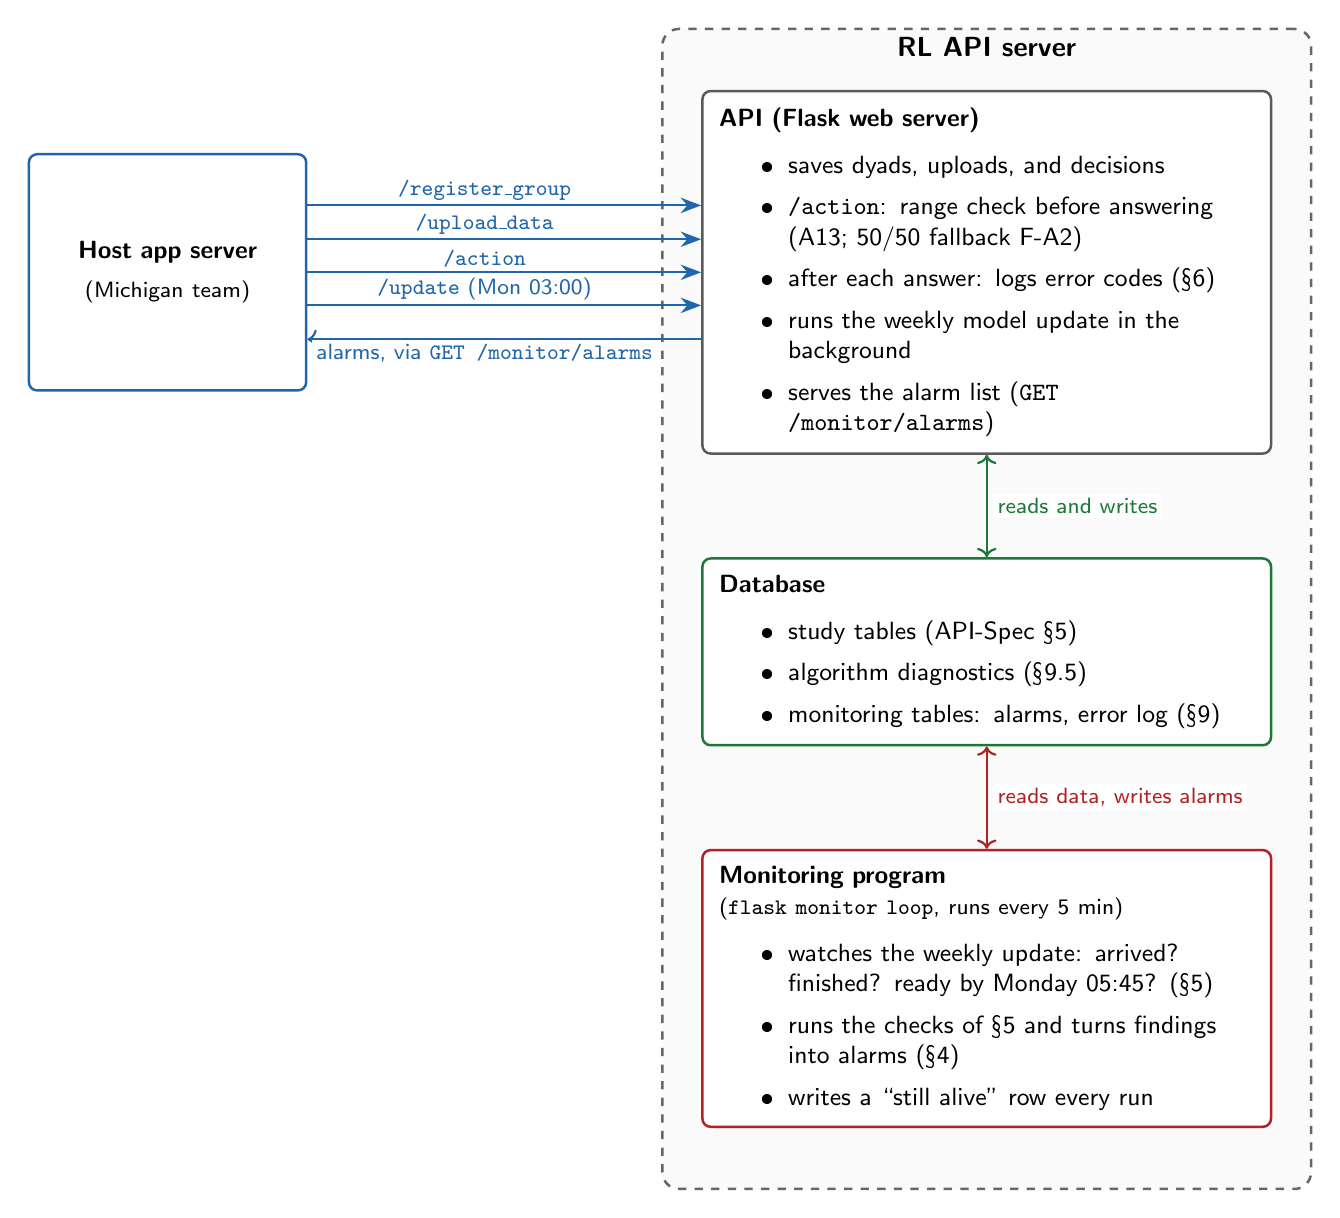
\begin{tikzpicture}[
  font=\sffamily\small,
  box/.style={draw, rounded corners=3pt, line width=0.9pt, align=left, inner sep=6pt, fill=white},
  title/.style={font=\sffamily\bfseries},
  arr/.style={-{Stealth[length=2.6mm]}, line width=0.8pt},
  lab/.style={font=\sffamily\footnotesize, fill=white, inner sep=1.5pt},
]

% ---------------- RL API server contents ----------------
\node[box, draw=apic, text width=6.8cm] (api) {%
  {\bfseries API (Flask web server)}\\[-2pt]
  \begin{itemize}
    \item saves dyads, uploads, and decisions
    \item \texttt{/action}: range check before answering (A13; 50/50 fallback F-A2)
    \item after each answer: logs error codes (\S6)
    \item runs the weekly model update in the background
    \item serves the alarm list (\texttt{GET /monitor/alarms})
  \end{itemize}};

\node[box, draw=dbc, text width=6.8cm, below=1.3cm of api] (db) {%
  {\bfseries Database}\\[-2pt]
  \begin{itemize}
    \item study tables (API-Spec \S5)
    \item algorithm diagnostics (\S9.5)
    \item monitoring tables: alarms, error log (\S9)
  \end{itemize}};

\node[box, draw=monc, text width=6.8cm, below=1.3cm of db] (mon) {%
  {\bfseries Monitoring program}\\
  {\footnotesize (\texttt{flask monitor loop}, runs every 5 min)}\\[-2pt]
  \begin{itemize}
    \item watches the weekly update: arrived? finished? ready by Monday 05:45? (\S5)
    \item runs the checks of \S5 and turns findings into alarms (\S4)
    \item writes a ``still alive'' row every run
  \end{itemize}};

\draw[arr, <->, dbc] (api.south) -- node[lab, right=2pt] {reads and writes} (db.north);
\draw[arr, <->, monc] (mon.north) -- node[lab, right=2pt] {reads data, writes alarms} (db.south);

% server frame
\begin{scope}[on background layer]
  \node[draw=black!60, dashed, rounded corners=6pt, line width=0.9pt,
        fit=(api)(db)(mon), inner xsep=14pt, inner ysep=22pt, fill=black!2] (server) {};
\end{scope}
\node[title, anchor=north] at (server.north) {RL API server};

% ---------------- Host ----------------
\node[box, draw=hostc, text width=3.1cm, align=center, minimum height=3.0cm,
      left=5.0cm of api.west, anchor=east] (host) {%
  {\bfseries Host app server}\\[3pt]\footnotesize (Michigan team)};

% host -> API calls
\coordinate (hA) at ($(host.east)+(0,0.85)$);
\coordinate (hB) at ($(host.east)+(0,0.42)$);
\coordinate (hC) at ($(host.east)+(0,0.0)$);
\coordinate (hD) at ($(host.east)+(0,-0.42)$);
\coordinate (hE) at ($(host.east)+(0,-0.85)$);

\draw[arr, hostc] (hA) -- node[lab, above, pos=0.45] {\texttt{/register\_group}} (hA -| api.west);
\draw[arr, hostc] (hB) -- node[lab, above, pos=0.45] {\texttt{/upload\_data}} (hB -| api.west);
\draw[arr, hostc] (hC) -- node[lab, above, pos=0.45] {\texttt{/action}} (hC -| api.west);
\draw[arr, hostc] (hD) -- node[lab, above, pos=0.45] {\texttt{/update} (Mon 03:00)} (hD -| api.west);
\draw[arr, hostc, <-] (hE) -- node[lab, below, pos=0.45] {alarms, via \texttt{GET /monitor/alarms}} (hE -| api.west);

\end{tikzpicture}
\end{document}
